\documentclass[twocolumn]{article}

\usepackage{imr}
\usepackage{graphicx}
\usepackage{amsfonts}
\usepackage{bbm}       % for \mathbbm{1}
\usepackage{amsmath}
\usepackage{mathrsfs}  % for \mathscr
\usepackage{minted}    % for including source code
\usepackage{tikz}
\usetikzlibrary{decorations.markings}

\def\thepage {}
\bibliographystyle{imr}

\newenvironment{smallarray}[1]
 {\null\,\vcenter\bgroup\scriptsize
  \renewcommand{\arraystretch}{0.7}%
  \arraycolsep=.13885em
  \hbox\bgroup$\array{@{}#1@{}}}
 {\endarray$\egroup\egroup\,\null}

\begin{document}

\title{Linear-algebraic representation and transformation of unstructured meshes}
\author{Daniel Shapero$^1$}
\date{
    $^1$University of Washington, Seattle, WA, USA, shapero@uw.edu
}

\abstract{This paper will show some new approaches for implementing common transformations to the connectivity or topology of an unstructured mesh.
The key enabling technology for our approach is to borrow ideas from algebraic topology: we use the \emph{boundary operators} of a \emph{chain complex} to represent the mesh.
Boundary operators are really just integer matrices.
By representing the objects of study using the language of linear algebra, we can use linear algebraic reasoning and intuition to define transformations.}

\keywords{mesh generation, computational geometry, algebraic topology}

\maketitle
\thispagestyle{empty}
\pagestyle{empty}


% --------------------
\section{Introduction}

Nearly all constructions in unstructured meshing require the ability to perform local transformations to the mesh topology.
For example, to compute the Delaunay triangulation, the Lawson algorithm uses a sequence of edge flips, while the Bowyer-Watson algorithm is based on splitting star-shaped polytopes along a vertex \cite{cheng2013delaunay}.
Algorithms for mesh coarsening, on the other hand, apply a sequence of edge or face collapses \cite{cignoni1998comparison}.
Implementing these low-level transformation kernels on common mesh data structures can be difficult and error-prone.
Are there other mesh data structures that make common algorithms easier to implement?

The idea of \emph{linear-algebraic representation} is to describe the mesh topology using a sequence of linear operators between certain vector spaces or modules.
The idea comes from algebraic topology: the linear operators are the \emph{boundary operators} on a certain \emph{chain complex}.
\textbf{If we can describe the mesh topology using linear algebra, then we can transform it using linear algebra as well.}
This viewpoint has been adopted in several publications on meshing and solid modeling \cite{dicarlo2007solid}, \cite{dicarlo2014linear}, \cite{mueller2017ternary}, \cite{paoluzzi2020topological}.
Other domains of science and engineering have seized on the idea of using linear algebra as the common language for building applications as well.
For example, the GraphBLAS project aims to implement common algorithms in graph theory using linear algebra \cite{mattson2013standards}.

This paper will show three transformations on the linear-algebraic represention of a polygonal mesh: (1) splitting a cell on a vertex, (2) merging adjacent cells, and (3) subdividing a cell along a collection of facets.
The main advantage of this linear-algebraic approach is that the transformation kernels are easy to write down and to code.
We show how other higher-level transformations can be implemented in terms of these primitive operations.
Finally, as a proof-of-concept, we implemented algorithms for computing convex hulls in arbitrary dimensions and constrained Delaunay triangulations in 2D.


% --------------
\section{Theory}

The mathematical theory that underlies the rest of the paper is basic algebraic topology.
We describe the connectivity of a mesh using the boundary operators on a finite, regular CW complex \cite{hatcher2002algebraic}.
The intuitive picture of a CW complex is a collection of cells or polygons that are attached together by certain maps.
The formal definition of a CW complex is inductive in the dimension.
A 0-dimensional complex $\Omega^0$ is a finite collection of points.
A finite $n$-dimensional complex consists of (1) an $n - 1$-dimensional complex $\Omega^{n - 1}$, and (2) a finite collection $\{\phi_\alpha^n\}$ of homeomorphisms called \emph{attaching maps} from the unit sphere $S^{n - 1}$ into $\Omega^{n - 1}$.
The complex $\Omega^n$ is then defined to be the disjoint union of copies of the unit ball, with the boundary of copy $\alpha$ identified with its image under the attaching map $\phi_\alpha^n$ under the quotient topology.
We will write $\Omega$ without a superscript for the whole complex, and $\Omega^k$ for the collection of all cells of dimension $k$.

The main character of our story is not the CW complex itself but rather the boundary operators between the chain modules.
To define what a boundary operator is we first need to describe what spaces it acts on.
A \emph{chain} $C$ is a formal integer linear combination of $k$-dimensional cells:
\begin{equation}
    C = c_1\sigma_1 + \ldots + c_m\sigma_m
\end{equation}
where the $c_i$ are integer coefficients and $\sigma_i$ are $k$-cells.
We write the space of all $k$-chains on a complex $\Omega$ as $\mathscr{C}^k(\Omega)$ or just $\mathscr{C}^k$ where the underlying CW complex is clear from context.

To define the boundary operators, we need some idea of orientation or incidence between cells.
For simplicial complexes, we define this orientation by picking orderings for how the vertices appear in each cell.
For cubical complexes, orientation is instead defined by deciding which faces are in the ``front'' or ``back'' along each axis.
There is no simple combinatorial definition of orientation or incidence for general CW complexes.
Instead, the definition requires some pre-existing notion of topological degree theory.
Let $\sigma$ be a $k$-cell of a complex and $\tau$ a $k - 1$-cell.
The quantity we wish to define is the \emph{incidence number} $[\sigma, \tau]$ between the two cells.
An intuitive definition of the incidence number is
\begin{equation}
    [\sigma, \tau] = \begin{cases}0 & \text{$\tau$ is not in $\sigma$} \\ +1 & \text{$\tau$ is positively-oriented in $\sigma$} \\ -1 & \text{$\tau$ is negatively oriented in $\sigma$}\end{cases}
\end{equation}
but this informal definition relies on some primitive idea of ``positive'' or ``negative'' orientation.
The formal definition of the incidence number relies on defining homology groups of spheres, the fact that maps between spaces can be pulled back to maps between homology groups, and the fact that the $n$-th homology group of the sphere $S^n$ is isomorphic to $\mathbb{Z}$.
Let $\phi$ be the map that attaches $\sigma$ into $\Omega$, and let $\phi^{-1}(\tau)$ be the pre-image of $\tau$ under this map.
Then the incidence number is defined formally as the topological degree of the attaching map $\phi$.
For our purposes, however, it is enough to think about incidence numbers using the informal definition.

We can now define the boundary operators.
The $k$-th boundary operator $\partial_k$ is a mapping from the $k$-chains to $k - 1$-chains:
\begin{equation}
    \partial_k : \mathscr{C}^k \to \mathscr{C}^{k - 1}.
\end{equation}
Given a $k$-cell $\sigma$, we define the boundary of $\sigma$ as
\begin{equation}
    \partial_k\sigma = \sum_{\tau \in \Omega^{k - 1}}[\sigma, \tau]\tau
\end{equation}
where the sum is over all $k - 1$-dimensional cells $\tau$.
We then extend the definition of $\partial_k$ to all of $\mathscr C^k$ by $\mathbb{Z}$-linearity.
The most important fact about boundary operators is that the boundary of a boundary is always equal to zero:
\begin{equation}
    \partial_k\cdot\partial_{k + 1} = 0.
    \label{eq:ddzero}
\end{equation}
This equation and its consequences is the starting point of homology theory, but we will not need to use this theory in the following.

There is one final definition that will clarify a later construction at a critical juncture.
The definitions above assume that the chain complex terminates at $\mathscr{C}^0$, i.e. integer linear combinations of the vertices or 0-dimensional cells.
We will instead include a single \emph{bottom} cell $\bot$ of dimension $-1$, together with a corresponding chain space $\mathscr{C}^{-1}$ which is isomorphic to $\mathbb{Z}$.
We then wish to define a 0-boundary operator $\partial_0 : \mathscr{C}^0 \to \mathscr{C}^{-1}$ such that $\partial_0\partial_1 = 0$.
We then define the boundary of any vertex $v$ to be $+\bot$; extending by linearity, the 0-boundary operator acts on the chain $\sum_kc_kv_k$ according to
\begin{equation}
    \partial_0\left(\sum_kc_kv_k\right) = \left(\sum_kc_k\right)\bot.
\end{equation}
In the algebraic topology literature, the inclusion of this bottom cell and chain space is used to form the \emph{reduced} homology groups.

Once we have chosen bases for the vector spaces $C^k$ and $C^{k - 1}$, we can represent the boundary operator $\partial_k$ as a matrix with integer entries.
These sparse integer matrices are the data structure that we will use to describe meshes and which we will perform transformations on.
The condition \eqref{eq:ddzero} is an invariant of this data structure.
Preserving this invariant constrains any transformations that we might define.

The matrix that represents the 0-boundary operator is the row vector of all 1s:
\begin{equation}
    \partial_0 = \mathbbm{1}^*.
    \label{eq:0-boundary-matrix}
\end{equation}
At a linear algebraic level, the condition that $\partial_0\partial_1 = 0$ now implies that the boundary of every edge has one positive and one negative vertex: $\partial e = v_i - v_j$ for some $i$, $j$.
We cannot have that, say, $\partial e = v_i + v_j$.
This outcome would be undesirable but no other condition on chain complexes explicitly forbids it.
Equation \eqref{eq:0-boundary-matrix} will reappear when we define the split transformation.


% -----------------------
\section{Transformations}

Here we will describe three different transformations that are easily implementable on the linear-algebraic representation of a mesh.
A \textbf{merge} operation combines several adjacent cells into one cell.
A \textbf{split} subdivides a cell into several cells along a new vertex.
A \textbf{bisection} subdivides a cell into several cells along a new facet or collection of facets.

Before showing the transformations themselves, it's worth considering some of the transformations of a chain complex that leave it unaltered.
First, observe that if $A$, $B$ are integer matrices such that the image of $\partial_{k + 1}$ is an invariant subspace of $A\cdot B$, then the matrices
\begin{equation}
    \partial_k' = \partial_k\cdot A, \quad \partial_{k + 1}' = B\cdot\partial_{k + 1}
\end{equation}
still satisfy $\partial_k'\cdot\partial_{k + 1}' = 0$.
A particular case is $A\cdot B = I$, which includes permutations of the cell ordering.
The more general case regarding the image of $A\cdot B$ is needed for some irreversible transformations.

\subsection{Merging}

A \emph{merge} of a set of $k$-cells replaces them with a single cell (provided that their union is simply-connected).
Merging is a column operation on the matrix $\partial_k$.
In the simplest case, the result column is the sum of all the columns to be merged, but in general we might need to flip some signs:
\begin{align}
    \partial_k' & = \partial_k\cdot\text{diag}(s_0, \ldots, s_m)\cdot\mathbbm{1}, \\
    \partial_{k + 1}' & = \left[\begin{matrix} 0 \ldots 1 \ldots 0\end{matrix}\right]\partial_{k + 1}. \label{eq:merge-k+1}
\end{align}
where $s_i$ are all $\pm 1$.
The signs are chosen so that any higher-dimensional cell $\sigma$ has the same incidence with respect to any of the cells $\tau$ to be merged.
The transformation to the rows of $\partial_{k + 1}$ collapses all incidence to any of the desired $k$-cells into incidence to the merged $k$-cell.
For merging cells of top dimension $n$, there are no higher-dimensional cells to apply equation \eqref{eq:merge-k+1} to and this step is left out.

\emph{Edge collapsing}, the key transformation in surface simplification algorithms \cite{gueziec1995surface}, is a merge of two vertices.


\subsection{Splitting}

A \emph{split} divides up the union of several polytopes along a vertex.
The key correctness criteria for this operation are that (1) every newly-created polytope contains the splitting vertex and (2) the boundary of the sum of all polytopes does not change.
This second condition can be expressed mathematically as
\begin{equation}
    \partial_k'\mathbbm{1} = \left[\begin{matrix}\partial_k\mathbbm{1} \\ 0\end{matrix}\right].
    \label{eq:split-preserves-boundaries}
\end{equation}
We'll describe the 2D case first and then proceed to arbitrary dimensions.

Suppose that a collection of adjacent polygons has the boundary operators $\partial_1$ and $\partial_2$.
We first have to draw edges between the new vertex and all the vertices of the polygon.
The orientation of these new edges is arbitrary, so we can assume that every edge goes from the splitting vertex $v$ to the polygon vertices.
Another way of stating this is that every new edge $e$ is negatively-incident to $v$ and positively-incident to some polygon vertex.
In terms of matrices, the new 1-boundary operator is
\begin{equation}
    \partial_1' = \left[\begin{matrix}\partial_1 & I \\ 0 & -\mathbbm{1}^*\end{matrix}\right]
    \label{eq:split-1-2d}
\end{equation}
where $I$ is the identity matrix.
The key step here is defining the 2-boundary matrix:
\begin{equation}
    \partial_2' = \left[\begin{matrix}\text{diag}(\partial_2\cdot\mathbbm{1}) \\ -\partial_1\cdot\text{diag}(\partial_2\cdot\mathbbm{1})\end{matrix}\right]
\end{equation}
A rudimentary calculation shows that $\partial_1'\partial_2' = 0$.
Since $\text{diag}(z)\cdot\mathbbm{1} = z$ for any vector $z$, we also find that
\begin{equation}
    \partial_2'\mathbbm{1} = \left[\begin{matrix}\partial_2\mathbbm{1} \\ 0\end{matrix}\right]
\end{equation}
which is exactly equation \eqref{eq:split-preserves-boundaries}, or that the new polygons have the same boundary as the old.
Figure \ref{fig:split-transformation} illustrates the split transformation on a single quadrilateral and shows the boundary matrices before and after.

\begin{figure}[h]
    \begin{center}
        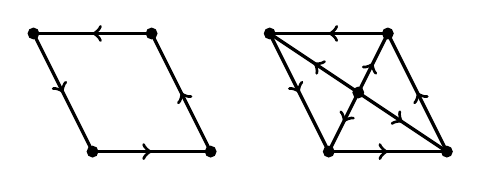
\begin{tikzpicture}[scale=0.75]
            \newcommand*{\defcoords}{
                \coordinate (p0) at (1.5, 1){};
                \coordinate (p1) at (1, 0){};
                \coordinate (p2) at (3, 0){};
                \coordinate (p3) at (2, 2){};
                \coordinate (p4) at (0, 2){};
            }

            \begin{scope}[
                very thick,
                decoration={markings, mark=at position 0.5 with {\arrow{>}}}
            ]
                \defcoords
                \draw[postaction={decorate}] (p1) -- (p2);
                \draw[postaction={decorate}] (p2) -- (p3);
                \draw[postaction={decorate}] (p3) -- (p4);
                \draw[postaction={decorate}] (p4) -- (p1);

                \foreach \p in {p1, p2, p3, p4} {
                    \filldraw (\p) circle (2pt);
                }
            \end{scope}

            \begin{scope}[
                very thick,
                shift={(4, 0)},
                decoration={markings, mark=at position 0.5 with {\arrow{>}}}
            ]
                \defcoords
                \draw[postaction={decorate}] (p1) -- (p2);
                \draw[postaction={decorate}] (p2) -- (p3);
                \draw[postaction={decorate}] (p3) -- (p4);
                \draw[postaction={decorate}] (p4) -- (p1);
                \draw[postaction={decorate}] (p0) -- (p2);
                \draw[postaction={decorate}] (p0) -- (p3);
                \draw[postaction={decorate}] (p0) -- (p4);
                \draw[postaction={decorate}] (p0) -- (p1);

                \foreach \p in {p0, p1, p2, p3, p4} {
                    \filldraw (\p) circle (2pt);
                }
            \end{scope}
        \end{tikzpicture}
    \end{center}

    \begin{equation*}
        \partial_1 = \left[\begin{smallmatrix}
            - &   &   & + \\
            + & - &   &   \\
              & + & - &   \\
              &   & + & -
        \end{smallmatrix}\right],
        \quad
        \partial_2 = \left[\begin{smallmatrix}
            + \\ + \\ + \\ +
        \end{smallmatrix}\right]
    \end{equation*}

    \begin{equation*}
        \partial_1' = \left[\begin{smallarray}{cccc|cccc}
            - &   &   & + & + &   &   &   \\
            + & - &   &   &   & + &   &   \\
              & + & - &   &   &   & + &   \\
              &   & + & - &   &   &   & + \\
            \hline
              &   &   &   & - & - & - & -
        \end{smallarray}\right], \quad
        \partial_2' = \left[\begin{smallarray}{cccc}
            + &   &   &   \\
              & + &   &   \\
              &   & + &   \\
              &   &   & + \\
            \hline
            + &   &   & - \\
            - & + &   &   \\
              & - & + &   \\
              &   & - & +
        \end{smallarray}\right]
    \end{equation*}

    \caption{Quadrilateral before and after splitting on a new vertex in the center (top) and boundary matrices before and after (bottom).}
    \label{fig:split-transformation}
\end{figure}

We can get an idea for how to extend this to $n$ dimensions by remembering the 0-boundary operator (equation \eqref{eq:0-boundary-matrix}).
In equation \eqref{eq:split-1-2d}, we can replace $\mathbbm{1}^* = \partial_0$.
This suggests the transformation
\begin{align}
    \partial_k' & = \left[\begin{matrix}\partial_k & I \\ 0 & -\partial_{k - 1}\end{matrix}\right] \label{eq:split-k} \\
    \partial_n' & = \left[\begin{matrix}\text{diag}(\partial_n\cdot\mathbbm{1}) \\ -\partial_{n - 1}\text{diag}(\partial_n\cdot\mathbbm{1})\end{matrix}\right] \label{eq:split-n}
\end{align}
Again, a rudimentary calculation shows that the fundamental equation \eqref{eq:ddzero} still holds and that the new polytopes have the same boundary as the old.

Equation \eqref{eq:split-k} has appeared before in the literature on homological algebra as the expression for the boundary operators of the \emph{cone} of a space \cite{gelfand1994homological}.
To our knowledge, using these equations for doing real computations is entirely new.

The Bowyer-Watson algorithm for Delaunay triangulation and all common algorithms for computing convex hulls only require the split transformation \cite{cheng2013delaunay}.

\subsection{Splitting and merging}

Other transformations can be defined by combining a sequence of splits and merges.
For example, figure \ref{fig:2-2-flip} shows how to perform a 2-2 flip in 2D by first splitting the quadrilateral into four triangles and then performing a sequence of merges and figure \ref{fig:2-3-flip} shows the same process for a 2-3 flip in 3D.
(We've shown an initial merge step for illustrative purposes, but this merge is actually part of the subsequent split.)

\begin{figure}[h]
    \tikzset{ec/.style={every coordinate/.try}}

    \begin{center}
    \begin{tikzpicture}[scale=0.4]
        \coordinate (p0) at (1.5, 1){};
        \coordinate (p1) at (1, 0){};
        \coordinate (p2) at (3, 0){};
        \coordinate (p3) at (2, 2){};
        \coordinate (p4) at (0, 2){};

        \begin{scope}[very thick]
            \draw (p1) -- (p2) -- (p4) -- cycle;
            \draw (p4) -- (p3) -- (p2) -- cycle;

            \foreach \p in {p1, p2, p3, p4} {
                \filldraw (\p) circle (3pt);
            }
        \end{scope}

        \begin{scope}[very thick, every coordinate/.style={shift={(3.5,0)}}]
            \draw ([ec]p1) -- ([ec]p2) -- ([ec]p3) -- ([ec]p4) -- cycle;

            \foreach \p in {p1, p2, p3, p4} {
                \filldraw ([ec]\p) circle (3pt);
            }
        \end{scope}

        \begin{scope}[very thick, every coordinate/.style={shift={(7,0)}}]
            \draw ([ec]p0) -- ([ec]p1) -- ([ec]p2) -- cycle;
            \draw ([ec]p0) -- ([ec]p2) -- ([ec]p3) -- cycle;
            \draw ([ec]p0) -- ([ec]p3) -- ([ec]p4) -- cycle;
            \draw ([ec]p0) -- ([ec]p4) -- ([ec]p1) -- cycle;

            \foreach \p in {p0, p1, p2, p3, p4} {
                \filldraw ([ec]\p) circle (3pt);
            }
        \end{scope}

        \begin{scope}[very thick, every coordinate/.style={shift={(10.5,0)}}]
            \draw ([ec]p1) -- ([ec]p2) -- ([ec]p3) -- cycle;
            \draw ([ec]p3) -- ([ec]p4) -- ([ec]p1) -- cycle;

            \foreach \p in {p0, p1, p2, p3, p4} {
                \filldraw ([ec]\p) circle (3pt);
            }
        \end{scope}

        \begin{scope}[very thick, every coordinate/.style={shift={(14,0)}}]
            \draw ([ec]p1) -- ([ec]p2) -- ([ec]p3) -- cycle;
            \draw ([ec]p3) -- ([ec]p4) -- ([ec]p1) -- cycle;

            \foreach \p in {p1, p2, p3, p4} {
                \filldraw ([ec]\p) circle (3pt);
            }
        \end{scope}

        \begin{scope}[very thick]
            \draw[->] (2, -0.2) arc[start angle=180, end angle=360, radius=1.5] node[midway, below, align=center] {merge\\triangles};
            \draw[->] (5.5, -0.2) arc[start angle=180, end angle=360, radius=1.5] node[midway, below] {split};
            \draw[->] (9.0, -0.2) arc[start angle=180, end angle=360, radius=1.5] node[midway, below, align=center] {merge\\triangles};
            \draw[->] (12.5, -0.2) arc[start angle=180, end angle=360, radius=1.5] node[midway, below, align=center] {merge\\edges};
        \end{scope}
    \end{tikzpicture}
    \end{center}
    \caption{A 2-2 flip, implemented as a sequence of merges and splits.
    The vertex added by splitting the quadrilateral is deleted when the two edges are merged in the final transformation.}
    \label{fig:2-2-flip}
\end{figure}

\begin{figure}[h]
    \begin{center}
        % Sketch output, version 0.3 (build 7d, Tue Aug 6 18:03:13 2024)
% Output language: PGF/TikZ,LaTeX
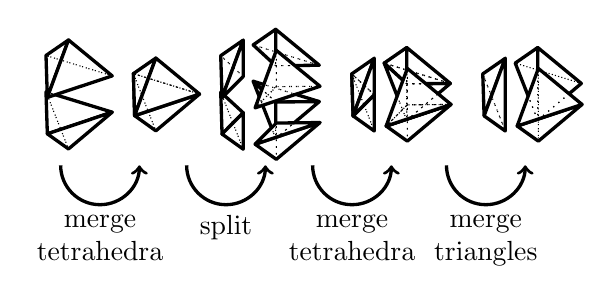
\begin{tikzpicture}[line join=round]
\filldraw[very thick,fill=white](2.631,-.096)--(2.345,.168)--(2.631,-.558)--cycle;
\filldraw[very thick,fill=white](3.185,-.091)--(2.345,.168)--(2.631,-.096)--cycle;
\filldraw[very thick,fill=white](2.631,-.558)--(3.185,-.091)--(2.631,-.096)--cycle;
\filldraw[very thick,fill=white](4.849,.14)--(4.009,.398)--(4.295,.135)--cycle;
\filldraw[very thick,fill=white](4.295,.596)--(4.009,.398)--(4.295,.135)--cycle;
\filldraw[very thick,fill=white](4.295,.135)--(4.009,.398)--(4.295,-.327)--cycle;
\filldraw[very thick,fill=white](5.673,.398)--(5.959,-.327)--(5.959,.596)--cycle;
\filldraw[very thick,fill=white](-.286,.033)--(-.269,-.5)--(.555,-.225)--cycle;
\filldraw[very thick,fill=white](1.933,.03)--(1.95,-.503)--(2.219,-.233)--cycle;
\filldraw[very thick,fill=white](4.295,-.327)--(4.849,.14)--(4.295,.135)--cycle;
\filldraw[very thick,fill=white](5.959,.596)--(5.959,-.327)--(6.513,.14)--cycle;
\filldraw[very thick,fill=white](.555,-.225)--(-.269,-.5)--(0,-.692)--cycle;
\filldraw[very thick,fill=white](2.219,-.233)--(1.95,-.503)--(2.219,-.695)--cycle;
\filldraw[very thick,fill=white](2.631,.827)--(2.345,.629)--(2.631,.365)--cycle;
\filldraw[very thick,fill=white](.824,.264)--(.84,-.269)--(1.664,.005)--cycle;
\filldraw[very thick,fill=white](.824,.264)--(.84,-.269)--(1.109,.462)--cycle;
\filldraw[very thick,fill=white](3.597,.261)--(3.614,-.272)--(3.883,-.003)--cycle;
\filldraw[very thick,fill=white](3.597,.261)--(3.614,-.272)--(3.883,.459)--cycle;
\filldraw[very thick,fill=white](5.261,.261)--(5.278,-.272)--(5.547,.459)--cycle;
\filldraw[very thick,fill=white](1.664,.005)--(.84,-.269)--(1.109,-.462)--cycle;
\filldraw[very thick,fill=white](3.883,-.003)--(3.614,-.272)--(3.883,-.464)--cycle;
\filldraw[very thick,fill=white](5.278,-.272)--(5.547,-.464)--(5.547,.459)--cycle;
\filldraw[very thick,fill=white](3.194,-.357)--(2.37,-.632)--(2.639,-.824)--cycle;
\filldraw[very thick,fill=white](-.286,.495)--(-.269,-.038)--(0,.692)--cycle;
\filldraw[very thick,fill=white](1.933,.492)--(1.95,-.041)--(2.219,.69)--cycle;
\filldraw[very thick,fill=white](4.295,.135)--(4.849,.14)--(4.295,.596)--cycle;
\filldraw[very thick,fill=white](4.858,-.127)--(4.034,-.401)--(4.303,-.593)--cycle;
\filldraw[very thick,fill=white](5.967,-.593)--(6.522,-.127)--(5.698,-.401)--cycle;
\filldraw[very thick,fill=white](2.631,.365)--(3.185,.371)--(2.631,.827)--cycle;
\filldraw[very thick,fill=white](1.109,.462)--(.84,-.269)--(1.664,.005)--cycle;
\filldraw[very thick,fill=white](3.883,.459)--(3.614,-.272)--(3.883,-.003)--cycle;
\filldraw[very thick,fill=white](2.37,-.632)--(3.194,-.357)--(2.639,-.363)--cycle;
\filldraw[very thick,fill=white](0,.692)--(-.269,-.038)--(.555,.236)--cycle;
\filldraw[very thick,fill=white](2.219,.69)--(1.95,-.041)--(2.219,.228)--cycle;
\filldraw[very thick,fill=white](4.034,-.401)--(4.858,-.127)--(4.303,-.132)--cycle;
\filldraw[very thick,fill=white](5.698,-.401)--(6.522,-.127)--(5.967,.33)--cycle;
\filldraw[very thick,fill=white](4.034,-.401)--(4.858,-.127)--(4.303,.33)--cycle;
\filldraw[very thick,fill=white](2.37,-.17)--(3.194,.104)--(2.639,.56)--cycle;
\filldraw[fill=none,dotted](-.286,.495)--(-.269,-.038)--(0,.692)--cycle;
\filldraw[fill=none,dotted](0,.692)--(-.269,-.038)--(.555,.236)--cycle;
\filldraw[fill=none,dotted](.555,.236)--(-.286,.495)--(0,.692)--cycle;
\filldraw[fill=none,dotted](-.269,-.038)--(-.286,.495)--(.555,.236)--cycle;
\filldraw[fill=none,dotted](-.269,-.5)--(-.286,.033)--(0,-.692)--cycle;
\filldraw[fill=none,dotted](0,-.692)--(-.286,.033)--(.555,-.225)--cycle;
\filldraw[fill=none,dotted](.555,-.225)--(-.269,-.5)--(0,-.692)--cycle;
\filldraw[fill=none,dotted](-.286,.033)--(-.269,-.5)--(.555,-.225)--cycle;
\filldraw[fill=none,dotted](.824,.264)--(.84,-.269)--(1.109,.462)--cycle;
\filldraw[fill=none,dotted](1.109,.462)--(.84,-.269)--(1.664,.005)--cycle;
\filldraw[fill=none,dotted](1.664,.005)--(.824,.264)--(1.109,.462)--cycle;
\filldraw[fill=none,dotted](.84,-.269)--(.824,.264)--(1.664,.005)--cycle;
\filldraw[fill=none,dotted](.84,-.269)--(.824,.264)--(1.109,-.462)--cycle;
\filldraw[fill=none,dotted](1.109,-.462)--(.824,.264)--(1.664,.005)--cycle;
\filldraw[fill=none,dotted](1.664,.005)--(.84,-.269)--(1.109,-.462)--cycle;
\filldraw[fill=none,dotted](.824,.264)--(.84,-.269)--(1.664,.005)--cycle;
\filldraw[fill=none,dotted](3.185,.371)--(2.345,.629)--(2.631,.827)--cycle;
\filldraw[fill=none,dotted](2.631,.827)--(2.345,.629)--(2.631,.365)--cycle;
\filldraw[fill=none,dotted](2.631,.365)--(3.185,.371)--(2.631,.827)--cycle;
\filldraw[fill=none,dotted](2.345,.629)--(3.185,.371)--(2.631,.365)--cycle;
\filldraw[fill=none,dotted](1.933,.492)--(1.95,-.041)--(2.219,.69)--cycle;
\filldraw[fill=none,dotted](2.219,.69)--(1.95,-.041)--(2.219,.228)--cycle;
\filldraw[fill=none,dotted](2.219,.228)--(1.933,.492)--(2.219,.69)--cycle;
\filldraw[fill=none,dotted](1.95,-.041)--(1.933,.492)--(2.219,.228)--cycle;
\filldraw[fill=none,dotted](2.37,-.17)--(3.194,.104)--(2.639,.56)--cycle;
\filldraw[fill=none,dotted](2.639,.56)--(3.194,.104)--(2.639,.099)--cycle;
\filldraw[fill=none,dotted](2.639,.099)--(2.37,-.17)--(2.639,.56)--cycle;
\filldraw[fill=none,dotted](3.194,.104)--(2.37,-.17)--(2.639,.099)--cycle;
\filldraw[fill=none,dotted](3.194,-.357)--(2.37,-.632)--(2.639,-.824)--cycle;
\filldraw[fill=none,dotted](2.639,-.824)--(2.37,-.632)--(2.639,-.363)--cycle;
\filldraw[fill=none,dotted](2.639,-.363)--(3.194,-.357)--(2.639,-.824)--cycle;
\filldraw[fill=none,dotted](2.37,-.632)--(3.194,-.357)--(2.639,-.363)--cycle;
\filldraw[fill=none,dotted](1.95,-.503)--(1.933,.03)--(2.219,-.695)--cycle;
\filldraw[fill=none,dotted](2.219,-.695)--(1.933,.03)--(2.219,-.233)--cycle;
\filldraw[fill=none,dotted](2.219,-.233)--(1.95,-.503)--(2.219,-.695)--cycle;
\filldraw[fill=none,dotted](1.933,.03)--(1.95,-.503)--(2.219,-.233)--cycle;
\filldraw[fill=none,dotted](2.345,.168)--(3.185,-.091)--(2.631,-.558)--cycle;
\filldraw[fill=none,dotted](2.631,-.558)--(3.185,-.091)--(2.631,-.096)--cycle;
\filldraw[fill=none,dotted](2.631,-.096)--(2.345,.168)--(2.631,-.558)--cycle;
\filldraw[fill=none,dotted](3.185,-.091)--(2.345,.168)--(2.631,-.096)--cycle;
\filldraw[fill=none,dotted](4.849,.14)--(4.009,.398)--(4.295,.596)--cycle;
\filldraw[fill=none,dotted](4.295,.596)--(4.009,.398)--(4.295,.135)--cycle;
\filldraw[fill=none,dotted](4.295,.135)--(4.849,.14)--(4.295,.596)--cycle;
\filldraw[fill=none,dotted](4.009,.398)--(4.849,.14)--(4.295,.135)--cycle;
\filldraw[fill=none,dotted](3.597,.261)--(3.614,-.272)--(3.883,.459)--cycle;
\filldraw[fill=none,dotted](3.883,.459)--(3.614,-.272)--(3.883,-.003)--cycle;
\filldraw[fill=none,dotted](3.883,-.003)--(3.597,.261)--(3.883,.459)--cycle;
\filldraw[fill=none,dotted](3.614,-.272)--(3.597,.261)--(3.883,-.003)--cycle;
\filldraw[fill=none,dotted](4.034,-.401)--(4.858,-.127)--(4.303,.33)--cycle;
\filldraw[fill=none,dotted](4.303,.33)--(4.858,-.127)--(4.303,-.132)--cycle;
\filldraw[fill=none,dotted](4.303,-.132)--(4.034,-.401)--(4.303,.33)--cycle;
\filldraw[fill=none,dotted](4.858,-.127)--(4.034,-.401)--(4.303,-.132)--cycle;
\filldraw[fill=none,dotted](4.858,-.127)--(4.034,-.401)--(4.303,-.593)--cycle;
\filldraw[fill=none,dotted](4.303,-.593)--(4.034,-.401)--(4.303,-.132)--cycle;
\filldraw[fill=none,dotted](4.303,-.132)--(4.858,-.127)--(4.303,-.593)--cycle;
\filldraw[fill=none,dotted](4.034,-.401)--(4.858,-.127)--(4.303,-.132)--cycle;
\filldraw[fill=none,dotted](3.614,-.272)--(3.597,.261)--(3.883,-.464)--cycle;
\filldraw[fill=none,dotted](3.883,-.464)--(3.597,.261)--(3.883,-.003)--cycle;
\filldraw[fill=none,dotted](3.883,-.003)--(3.614,-.272)--(3.883,-.464)--cycle;
\filldraw[fill=none,dotted](3.597,.261)--(3.614,-.272)--(3.883,-.003)--cycle;
\filldraw[fill=none,dotted](4.009,.398)--(4.849,.14)--(4.295,-.327)--cycle;
\filldraw[fill=none,dotted](4.295,-.327)--(4.849,.14)--(4.295,.135)--cycle;
\filldraw[fill=none,dotted](4.295,.135)--(4.009,.398)--(4.295,-.327)--cycle;
\filldraw[fill=none,dotted](4.849,.14)--(4.009,.398)--(4.295,.135)--cycle;
\filldraw[fill=none,dotted](5.673,.398)--(5.959,-.327)--(5.959,.596)--cycle;
\filldraw[fill=none,dotted](5.959,.596)--(5.959,-.327)--(6.513,.14)--cycle;
\filldraw[fill=none,dotted](6.513,.14)--(5.673,.398)--(5.959,.596)--cycle;
\filldraw[fill=none,dotted](5.959,-.327)--(5.673,.398)--(6.513,.14)--cycle;
\filldraw[fill=none,dotted](5.278,-.272)--(5.547,-.464)--(5.547,.459)--cycle;
\filldraw[fill=none,dotted](5.547,.459)--(5.547,-.464)--(5.261,.261)--cycle;
\filldraw[fill=none,dotted](5.261,.261)--(5.278,-.272)--(5.547,.459)--cycle;
\filldraw[fill=none,dotted](5.547,-.464)--(5.278,-.272)--(5.261,.261)--cycle;
\filldraw[fill=none,dotted](6.522,-.127)--(5.967,-.593)--(5.967,.33)--cycle;
\filldraw[fill=none,dotted](5.967,.33)--(5.967,-.593)--(5.698,-.401)--cycle;
\filldraw[fill=none,dotted](5.698,-.401)--(6.522,-.127)--(5.967,.33)--cycle;
\filldraw[fill=none,dotted](5.967,-.593)--(6.522,-.127)--(5.698,-.401)--cycle;

\begin{scope}[very thick]
    \draw[->] (-0.1, -0.9) arc[start angle=180, end angle=360, radius=0.5] node[midway, below, align=center] {merge\\tetrahedra};
    \draw[->] (1.5, -0.9) arc[start angle=180, end angle=360, radius=0.5] node[midway, below, align=center] {split};
    \draw[->] (3.1, -0.9) arc[start angle=180, end angle=360, radius=0.5] node[midway, below, align=center] {merge\\tetrahedra};
    \draw[->] (4.8, -0.9) arc[start angle=180, end angle=360, radius=0.5] node[midway, below, align=center] {merge\\triangles};
\end{scope}
\end{tikzpicture}% End sketch output

    \end{center}
    \caption{A 2-3 flip implemented as a sequence of merges and splits.
    We've shown the tetrahedra in an ``exploded'' view to help with visualization.}
    \label{fig:2-3-flip}
\end{figure}

\textcolor{red}{This text is copied over from the short paper but it needs revisiting.
The current paper is supposed to do or at least enable multi-face retriangulation so we need to be less speculative and prove the concept.}
A few papers have proposed using multi-cell transformations for 3D mesh improvement \cite{klingner2008aggressive}.
Multi-cell transformations are more complex than 2-3 or 3-2 flips, but \cite{misztal2009tetrahedral} showed that they can be implemented as a sequence of flips.
Using the boundary operators might make it possible to implement complex transformations with less effort.
The split transformation that we derived here is based on computing the topological cone of a space and then removing the base of the cone.
Multiface retriangulation, as advocated in \cite{misztal2009tetrahedral}, is a transformation of a \emph{suspension}, a related construction in algebraic topology \cite{hatcher2002algebraic}.

\subsection{Bisection}

Finally, we consider the problem of how to split a single $k$-cell $P$ into two or more cells along a collection of $(k - 1)$-cells.
In order to be able to split the top cell, we need to assume a certain connectivity structure between its faces.
A $k$-\emph{path} in $\Omega$ is a collection $\{f_0, s_0, f_1, s_1, \ldots, f_{m - 1}, s_{m - 1}, f_m\}$ such that $s_i$ is a common sub-face of both $f_i$ and $f_{i + 1}$ for each $i$.
Given two collections of faces $F_1$, $F_2$, we say that a third collection of faces $F$ is a \emph{separator} for $F_1$, $F_2$ if any path from a cell $f_1$ in $F_1$ to a cell $f_2$ in $F_2$ must include some cell $f$ in $F$.
The definition is similar to that of graph theory but with some important differences in the case of cell complexes.

In order to be able to subdivide $P$ into multiple cells, we need to be able to partition its faces into two or more groups $\{F_1, \ldots, F_m\}$ with a common separator $F_0$.
Moreover, we assume at first that $[P, F_0] = 0$ and $[P, F_i] \neq 0$ for $i \ge 1$.
We can find separators and subgroups through a procedure analogous to breadth-first search but with adjacency defined by sharing common subfaces.

The boundary matrices at first will have the form
\begin{equation}
    \partial_k = \Big[\begin{matrix}[S, F_0] & [S, F_1] & \cdots & [S, F_m]\end{matrix}\Big],
\end{equation}
where $S$ denotes the set of all subfaces or $k - 2$-dimensional cells contained in $P$, and
\begin{equation}
    \partial_{k + 1} = \left[\begin{matrix} 0 \\ [F_1, P] \\ \vdots \\ [F_m, P]\end{matrix}\right].
\end{equation}
The fundamental equation \eqref{eq:ddzero} then implies that
\begin{equation}
    \sum_i[S, F_i]\cdot[F_i, P] = 0.
\end{equation}
We then make the ansatz that the transformed boundary matrix will have the form
\begin{equation}
    \partial_{k + 1}' = \left[\begin{matrix}[F_0, P_1] & \cdots & [F_0, P_m] \\ [F_1, P] & & \\ & \ddots & \\ & & [F_m, P]\end{matrix}\right]
\end{equation}
where the adjacencies $[F_0, P_i]$ need to be solved for.
Provided that $\sum_i[F_0, P_i]\mathbbm{1} = 0$, the boundary of the new chain will be the same as the old.
To preserve the fundamental equation $\partial\partial = 0$, we need that
\begin{equation}
    [S, F_0][F_0, P_i] = -[S, F_i][F_i, P].
\end{equation}
We can then attempt to find a solution of this collection of linear systems of equations.
The existence of a solution is not guaranteed a priori, but if we can find one then it defines a valid subdivision of the original cell.
The system is also rectangular, so it may be under- or over-determined depending on the number of faces and subfaces.
We can obtain a square system by instead opting to solve
\begin{equation}
    [S, F_0]^*[S, F_0][F_0, P_i] = -[S, F_0]^*[S, F_i][F_i, P].
\end{equation}
We can compute solutions to integer linear systems by first finding the Hermite normal form of the system matrix \cite{kannan1979polynomial}.


% ---------------------
\section{Demonstration}

As a proof of concept, we developed a software package called \emph{topomesh} which implements the transformations defined above.
We then implemented several common algorithms in computational geometry using these transformations.

\subsection{Splitting and convex hulls}

The split transformation is the key computational kernel for computing convex hulls in any dimension.
The source code for the split transformation is shown in figure \ref{fig:split-source-code}.
\begin{figure}
    \begin{minted}[fontsize=\footnotesize,linenos]{python}
import numpy as np
from typing import List

def split(D: List[np.ndarray]) -> List[np.ndarray]:
    # Create the boundary matrices for 1 <= k < n
    n_vertices = D[0].shape[1]
    E = [np.ones((1, n_vertices + 1), int)]
    for k in range(1, len(D) - 1):
        n_cells = D[k].shape[1]
        n_sub_faces, n_faces = D[k - 1].shape
        I = np.identity(n_faces, int)
        Z = np.zeros((n_sub_faces, n_cells), int)
        E_k = np.block([[D[k], I], [Z, -D[k - 1]]])
        E.append(E_k)

    # Create the top-dimensional boundary matrix
    C = np.diag(np.sum(D[-1], axis=1))
    E_n = np.vstack((C, -D[-2] @ C))
    E.append(E_n)
    return E
    \end{minted}
    \caption{Python source code for the split transformation.
    Line 13 corresponds to equation \eqref{eq:split-k}; lines 17 and 18 correspond to equation \eqref{eq:split-n}.
    The real version has some additional logic to remove empty cells.}
    \label{fig:split-source-code}
\end{figure}

We used the split transformation to implement a convex hull algorithm that works in arbitrary dimensions.
To test the convex hull code, we used (1) random point sets up to dimension 5 and (2) several synthetic input sets with various degeneracies such as coplanarity.
For geometric predicates, we used interval arithmetic and fall back to exact rational arithmetic if the result interval contains zero.
\textcolor{red}{Elaborate...}

Our implementation of the convex hull algorithm takes in a function as argument which supplies the procedure for computing the signed volume predicate.
Computing Delaunay triangulations is equivalent to computing the lower half of a convex hull of the input points lifted to a paraboloid.
We also implemented a Delaunay triangulation method which reuses our convex hull algorithm by supplying an insphere function instead of the usual signed volume function.


\subsection{Constrained Delaunay triangulation}

The split transformation alone is enough to compute convex hulls and unconstrained Delaunay triangulations.
Computing a constrained Delaunay triangulation (CDT), on the other hand, requires both merges and bisections.
We implemented a CDT algorithm based on \cite{anglada1997improved}.
\textcolor{red}{Elaborate...}


% ------------------
\section{Conclusion}

Doubly-connected edge lists have historically been popular for mesh generation because they offer a simple interface for traversing the topology \cite{guibas1985primitives}.
Here we propose that boundary operators are an ideal representation if the goal is to perform topological transformations.
This idea has appeared before, for example in the work of DiCarlo and others \cite{dicarlo2007solid}.

Boundary operators are only necessary for representing a small patch of the topology at a time.
Once the transformed patch is computed, it can be translated back to a set of simplexes.
Boundary operators are useful for describing non-simplicial intermediate states of a transformation; they are not space-optimal for describing an entire simplicial complex.

When the objects of study can be represented as linear operators, we can apply linear algebraic reasoning to define transformations and verify that they preserve all of the important invariants.
The condition in equation \eqref{eq:ddzero} that the product of two boundary operators is zero is a powerful invariant for ensuring the validity of the underlying topology.


\bibliography{chain-complexes.bib}

\end{document}
